\section{Method}

The following section outlines the structure of the project, from theoretical formulation, to data acquisition, to lab testing, to deployment. 
The camera pipeline is first developed in a simulated environment, with spectral transmission functions acquired from producer specifications and camera sensitivity functions acquired in the same way. 
Thus, a full simulation of our camera can be deployed on multispectral image sets and tested in our filter selection harness.
Later, measurements of a subset of filters are taken in the lab, a measurement of camera spectral sensitivity function is also done in the same controlled lighting environment as the filter measurements, and captures are taken of a Preferred Memory Color Chart (PMCC) for quantitative analysis. 

\subsection{Mathematical Framework}

%%%% Alternate Math - Graham
In our model we have a single grey-scale camera (only a brightness channel). Thus, our estimated new camera sensitivities are a function of the intrinsic sensitivities of this single channel camera multiplied by the filter transmittances.
Let ${f}_k(\lambda)$ and $\boldsymbol{M}_c$ respectively denote $k$ filter functions multiplied by the camera sensor response and the $c$'th row of a $3 \times k$ matrix that linearly combines these filter functions (e.g. to best approximate the XYZ color matching functions). 
Then the filtered color response, ${\rho}_{c,k}$ is written as:


\begin{equation}
{\rho}_{c,k}=\int_\omega \mathbf{M}_c{f}_k(\lambda)E(\lambda)S(\lambda)d\lambda
\end{equation}

Where $E(\lambda)$ is the spectral reflectance function and $S(\lambda)$ is the camera spectral sensitivity function. 

%The function $\rho'_c(\lambda)$ denotes a single estimated camera sensor where $c\in \{R,G,B\}$, $\rho'_c(\lambda)=\mathbf{M}_c\underline{f}(\lambda)$, where ${M}_c$ denotes the corresponding row of $\mathbf{M}$.
In the optimizations that follow, we will solve for the R, G and B sensors that best approximate the actual X, Y and Z color matching function sensitivities, respectively referred to as $X_c \in \{X,Y,Z\}$.

%%%%%% end of alternate math 

%We define our camera's response for color channel $c\in \{R,G,B\}$ as the integral dot product between the corresponding row of $\boldsymbol{M}$ (defined $M_c$) and our selected filters' transmission functions $\underline{f}(\lambda)$.
%Decomposing our camera's sensitivity function over the $c$'th color channel $Q_c(\lambda)$ we have: 
%\begin{equation}
  %  \rho_{c} = \int_{\omega} M_c\underline{f}(\lambda)E(\lambda)S(\lambda) d\lambda
  %  \label{eq:2}
%\end{equation}
%And we define the integrand $\rho'_c$ as:
%\begin{equation}
 %   \rho'_{c}(\lambda) = M_c\underline{f}(\lambda)E(\lambda)S(\lambda)
 %   \label{eq:3}
%\end{equation}



\subsection{Data Collection}
The aim of our method is to capture multiple images through different color filters and then combine them to match the colors of an image of a scene captured with respect to the CIE XYZ color matching functions (CMFs). 
We will choose filters drawn from a set of Rosco Supergel filters that we measure in our lab. 
We model our camera's and optional NOIR filter's spectral response function as per the manufacturer's specifications \cite{arducam_ov9281, coligh_ircut_650nm}
All filters are represented in the domain $\omega = [400,750]$ nm. 

First, we gather a set of 494 filters from the Rosco Supergel MyColor tool \cite{rosco_mycolor}. 
Rosco provides a specification sheet and spectral response function for each filter in the MyColor catalog.

\begin{figure}[H]
    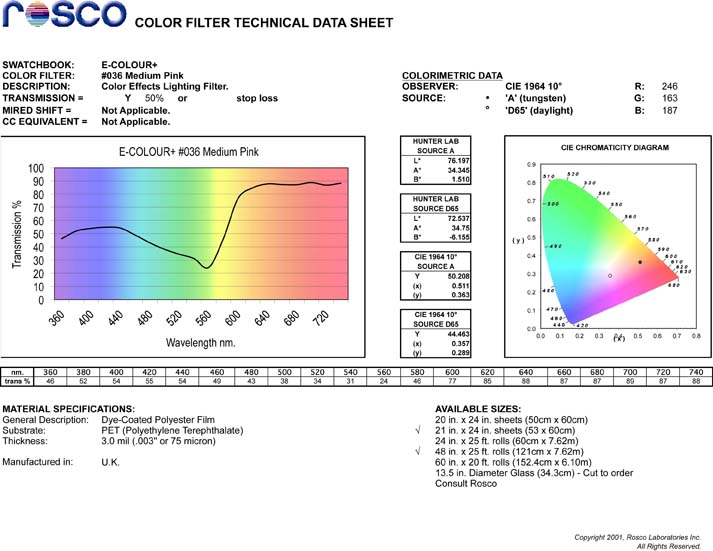
\includegraphics[width=\linewidth]{media/E036_Spec.jpg}
    \caption{Specification Sheet for Filter 'E036'}
\end{figure}

We utilize a web scraping script to pull the spec sheets of all 494 filters from the MyColor tool and approximate the spectral response functions from the chart. 
We compute a transmission function estimate from the attached spec sheet for each filter, and save the transmittance at each discrete wavelength $\lambda$ within $\omega$ denoted as $\omega_d = \{400,401,...750\}$

\begin{figure}[H]
    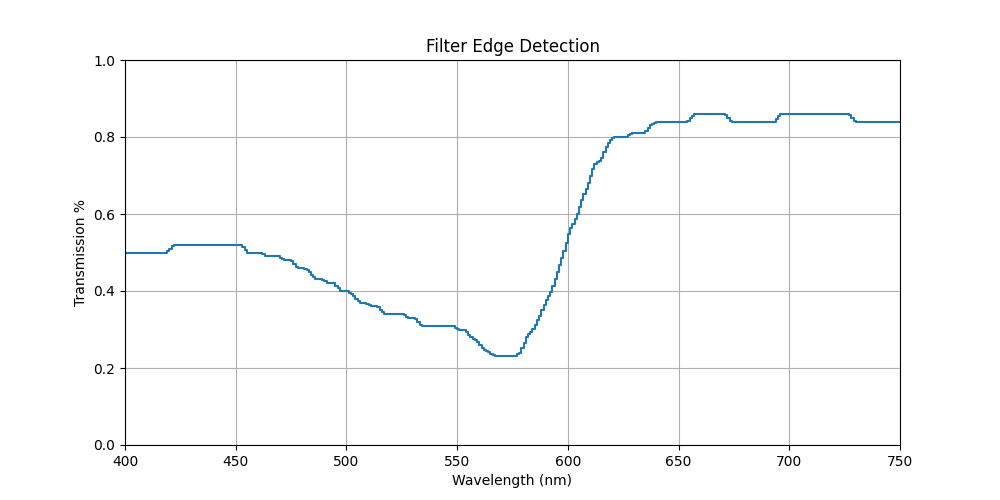
\includegraphics[width=\linewidth]{media/E036.png}
    \caption{Spectral transmission function for $\lambda \in \omega_d$ for MyColor tool filter 'E306'}
\end{figure}

We utilize a similar approach for our simulated camera, acquired from Arducam \cite{arducam_ov9281}. 
The various specification sheets generally provide full cover over $\omega_d$. 

\begin{figure}[H]
    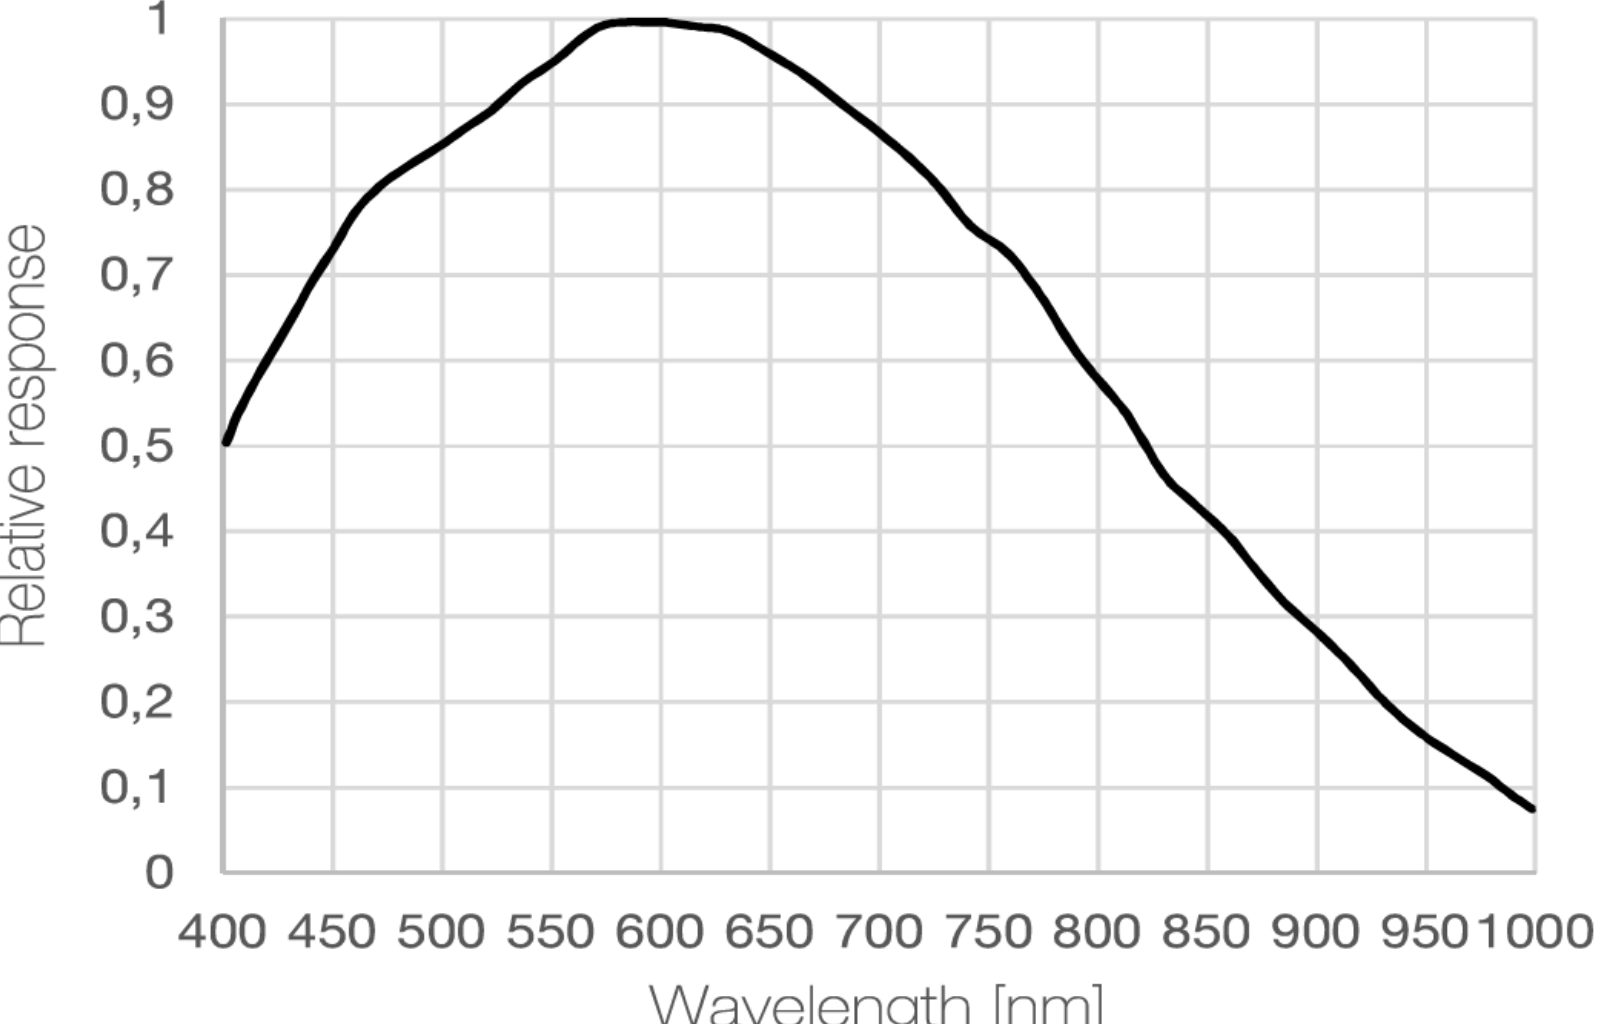
\includegraphics[width=\linewidth]{media/RaspberryPi_trans.png}
    \caption{Monochrome camera transmission function for $\lambda \in [400,1000]$}
\end{figure}

The simulated set of 494 filters from the MyColor tool cover a large space, useful for finding a best-case-scenario when nearly unconstrained by transmission function. 
In reality, we have a set of 119 filters to choose from, which will be sufficient for practical results.
We use a dark room, Lilliput lamp \cite{UtopiaCamLiliput}, and a spectrophotometer to measure the transmission functions of our set of filters. 

\begin{figure}[H]
    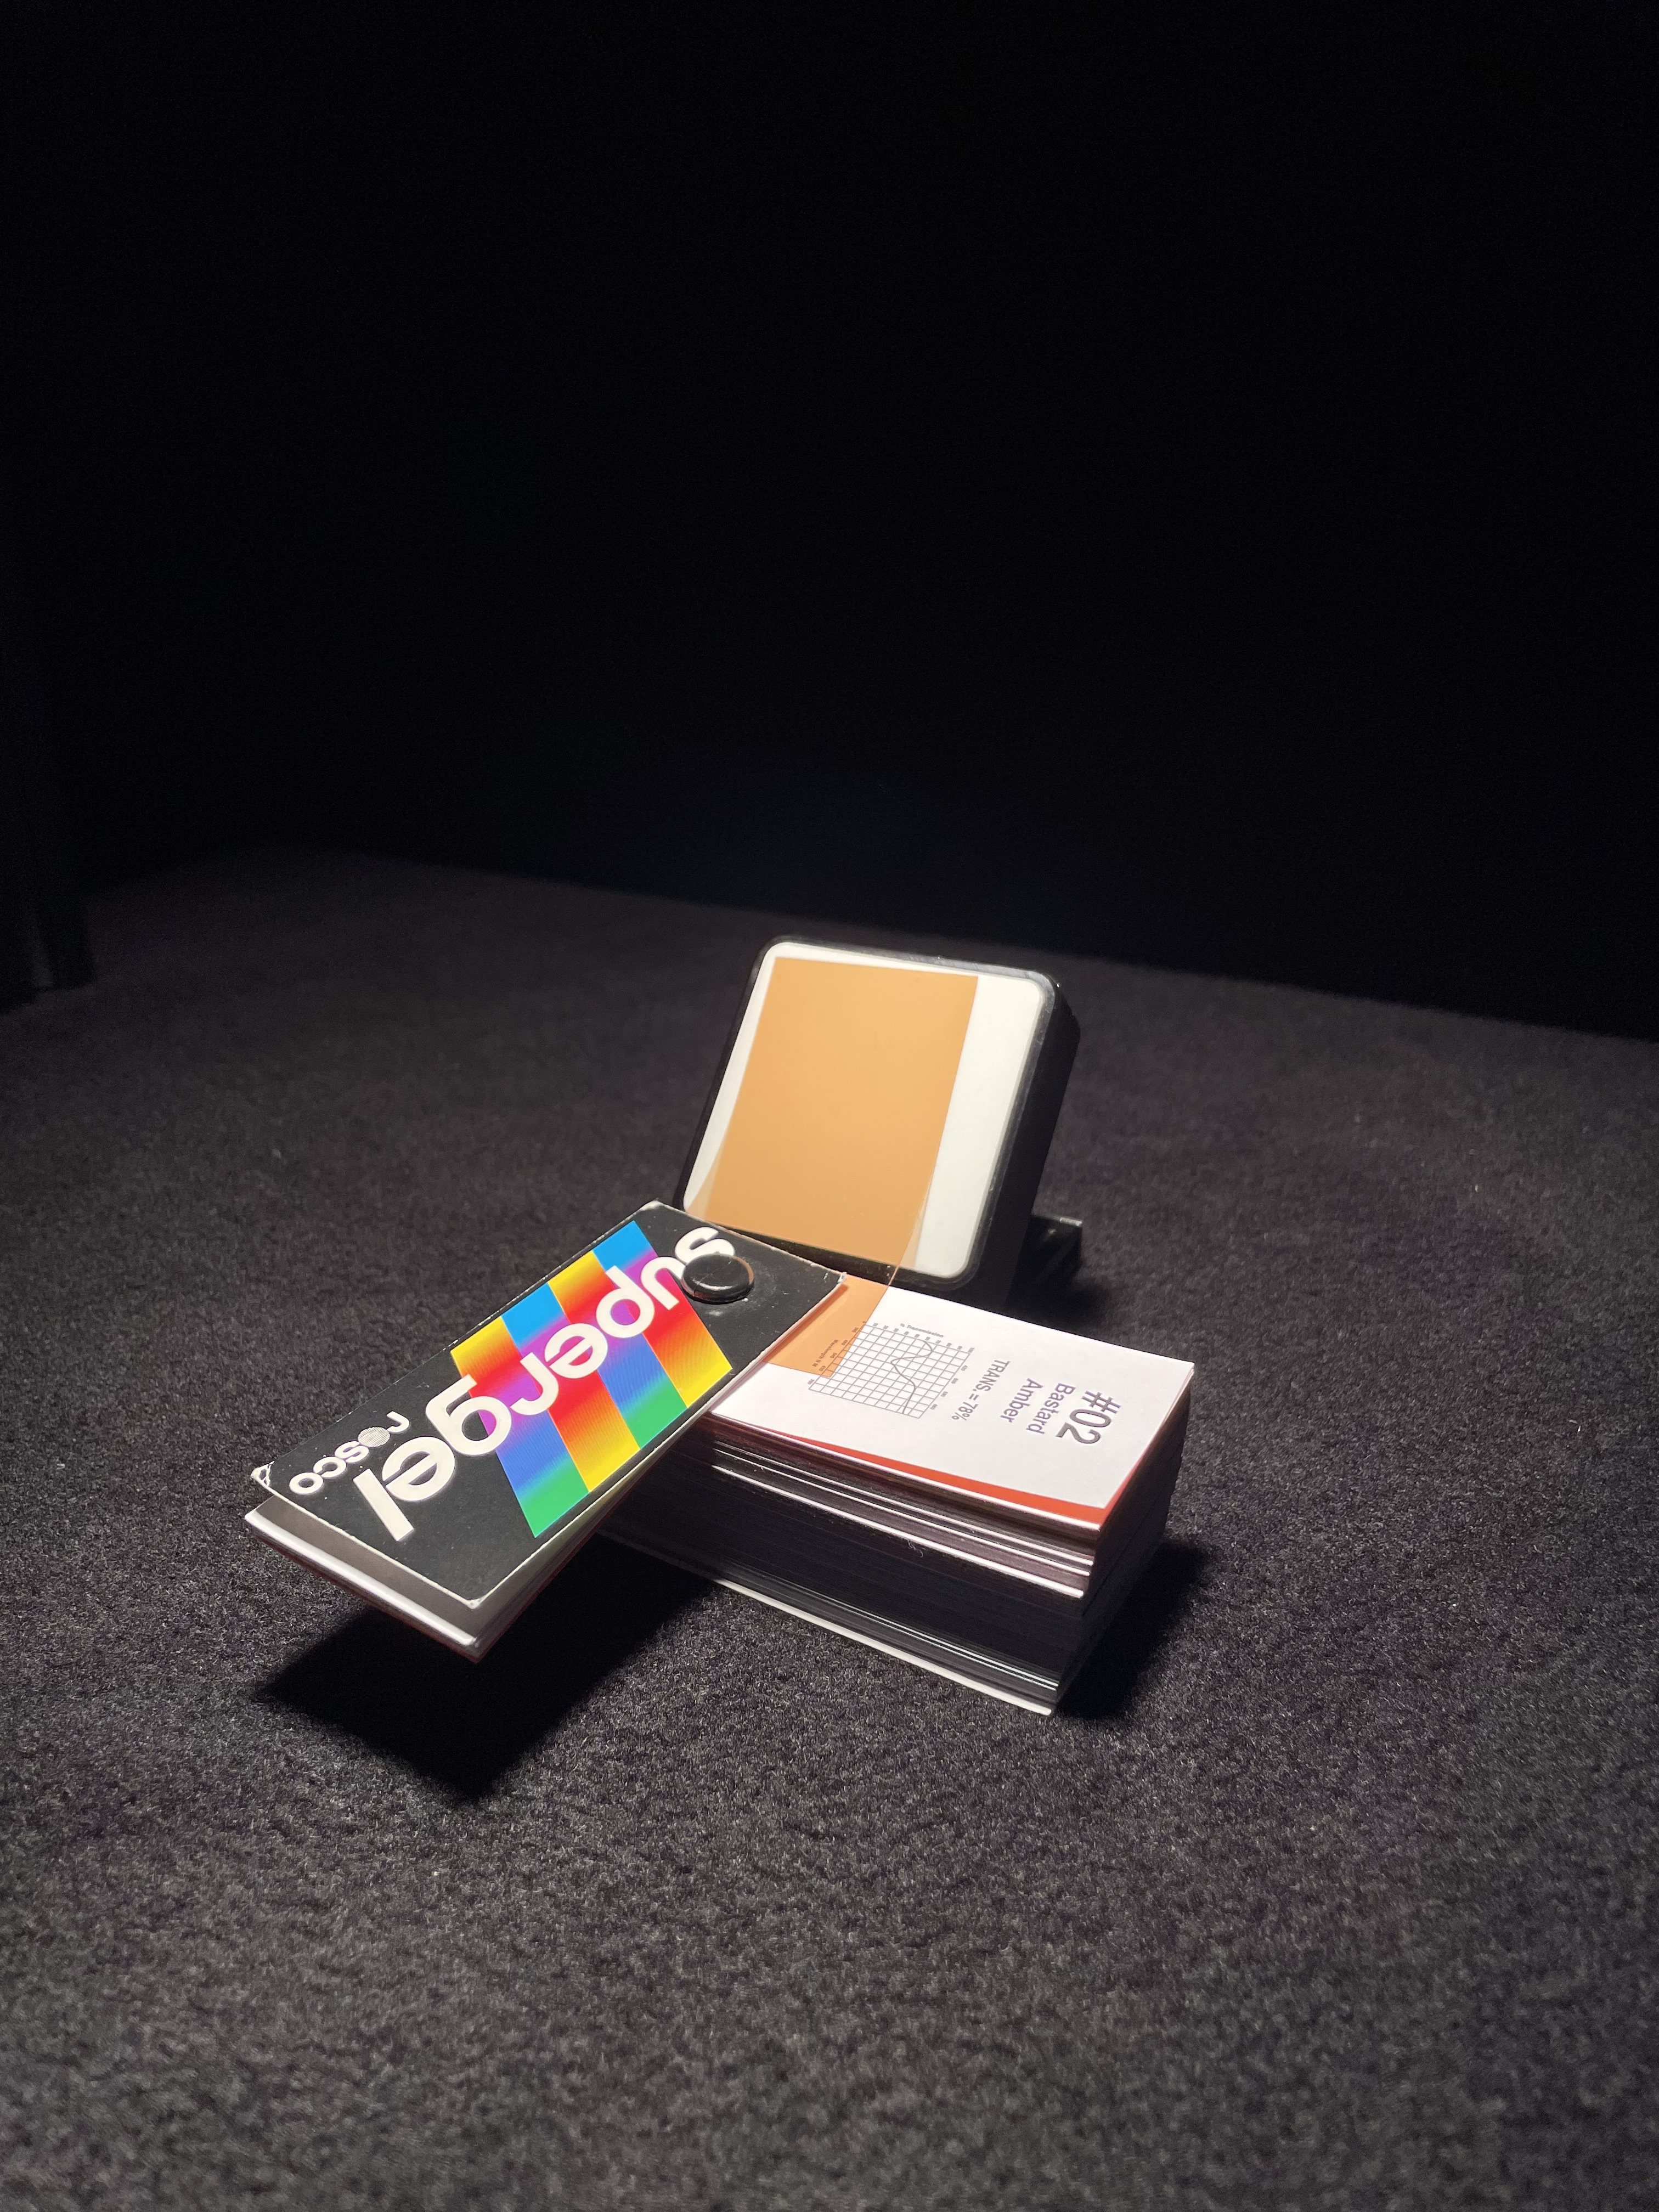
\includegraphics[width=\linewidth]{media/Gels.jpeg}
    \caption{Set of 119 Supergel Filters with \#02 on stage}
\end{figure}

We set up a stage consisting of an overhead illuminant, a reflective surface placed at a 45º angle, and a spectrophotometer pointed at the stage. 
The stage is placed at a 45º angle to the lamp above, with the spectrophotometer aimed at a flush angle to the stage.
The spectrophotometer takes a luminance reading at each wavelength from 350-1000, as well as a measurement of $x$ and $y$, from which the XYZ color coordinates may be derived. 
For this case, we are interested in calculating the transmission function of each filter, so we care about the luminance reading, but further applications of the spectrophotometer, specifically the $x$ and $y$ reading will be discussed below. 

\begin{figure}[H]
    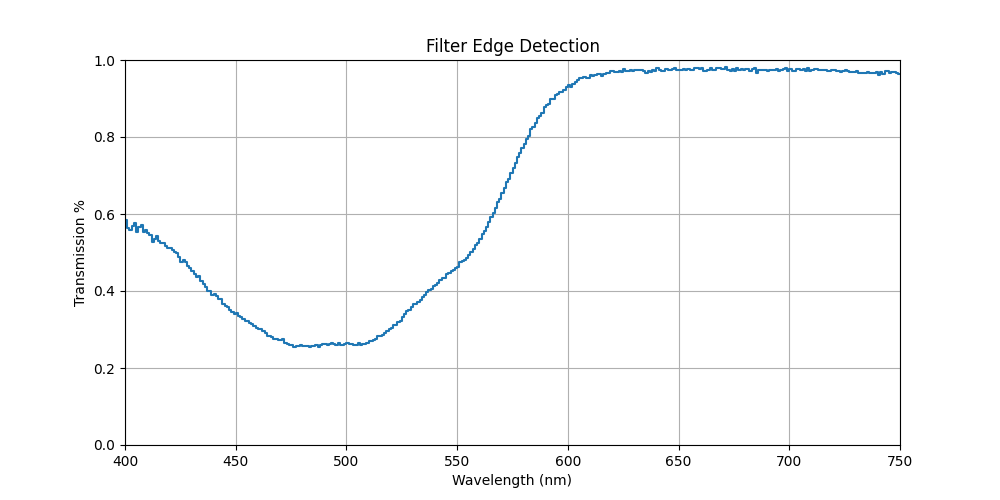
\includegraphics[width=\linewidth]{media/304.png}
    \caption{Measurement of Supergel filter \#304 for $\lambda \in \omega_d$}
\end{figure}

Brightness in the room was controlled by covering the walls with black felt and ensuring that the computer monitor was pointed away from the stage. 
The spectrophotometer is equipped with a laser to ensure accuracy in measurement, and each filter was placed flush against the stage for measurement. 

\begin{figure}[H]
    \includegraphics[width=\linewidth]{media/measure2labeled.jpeg}
    \caption{Filter measurement setup with spectrophotometer and Rosco Supergel filters.}
\end{figure}

The stage and illuminant can be seen on the left below, with the control panel and transmission function readout on the right. 
The results of each scan are saved into a $.mat$ file at 1 nanometer increments, along with a few calibration runs with no filter present.

\begin{figure}[H]
    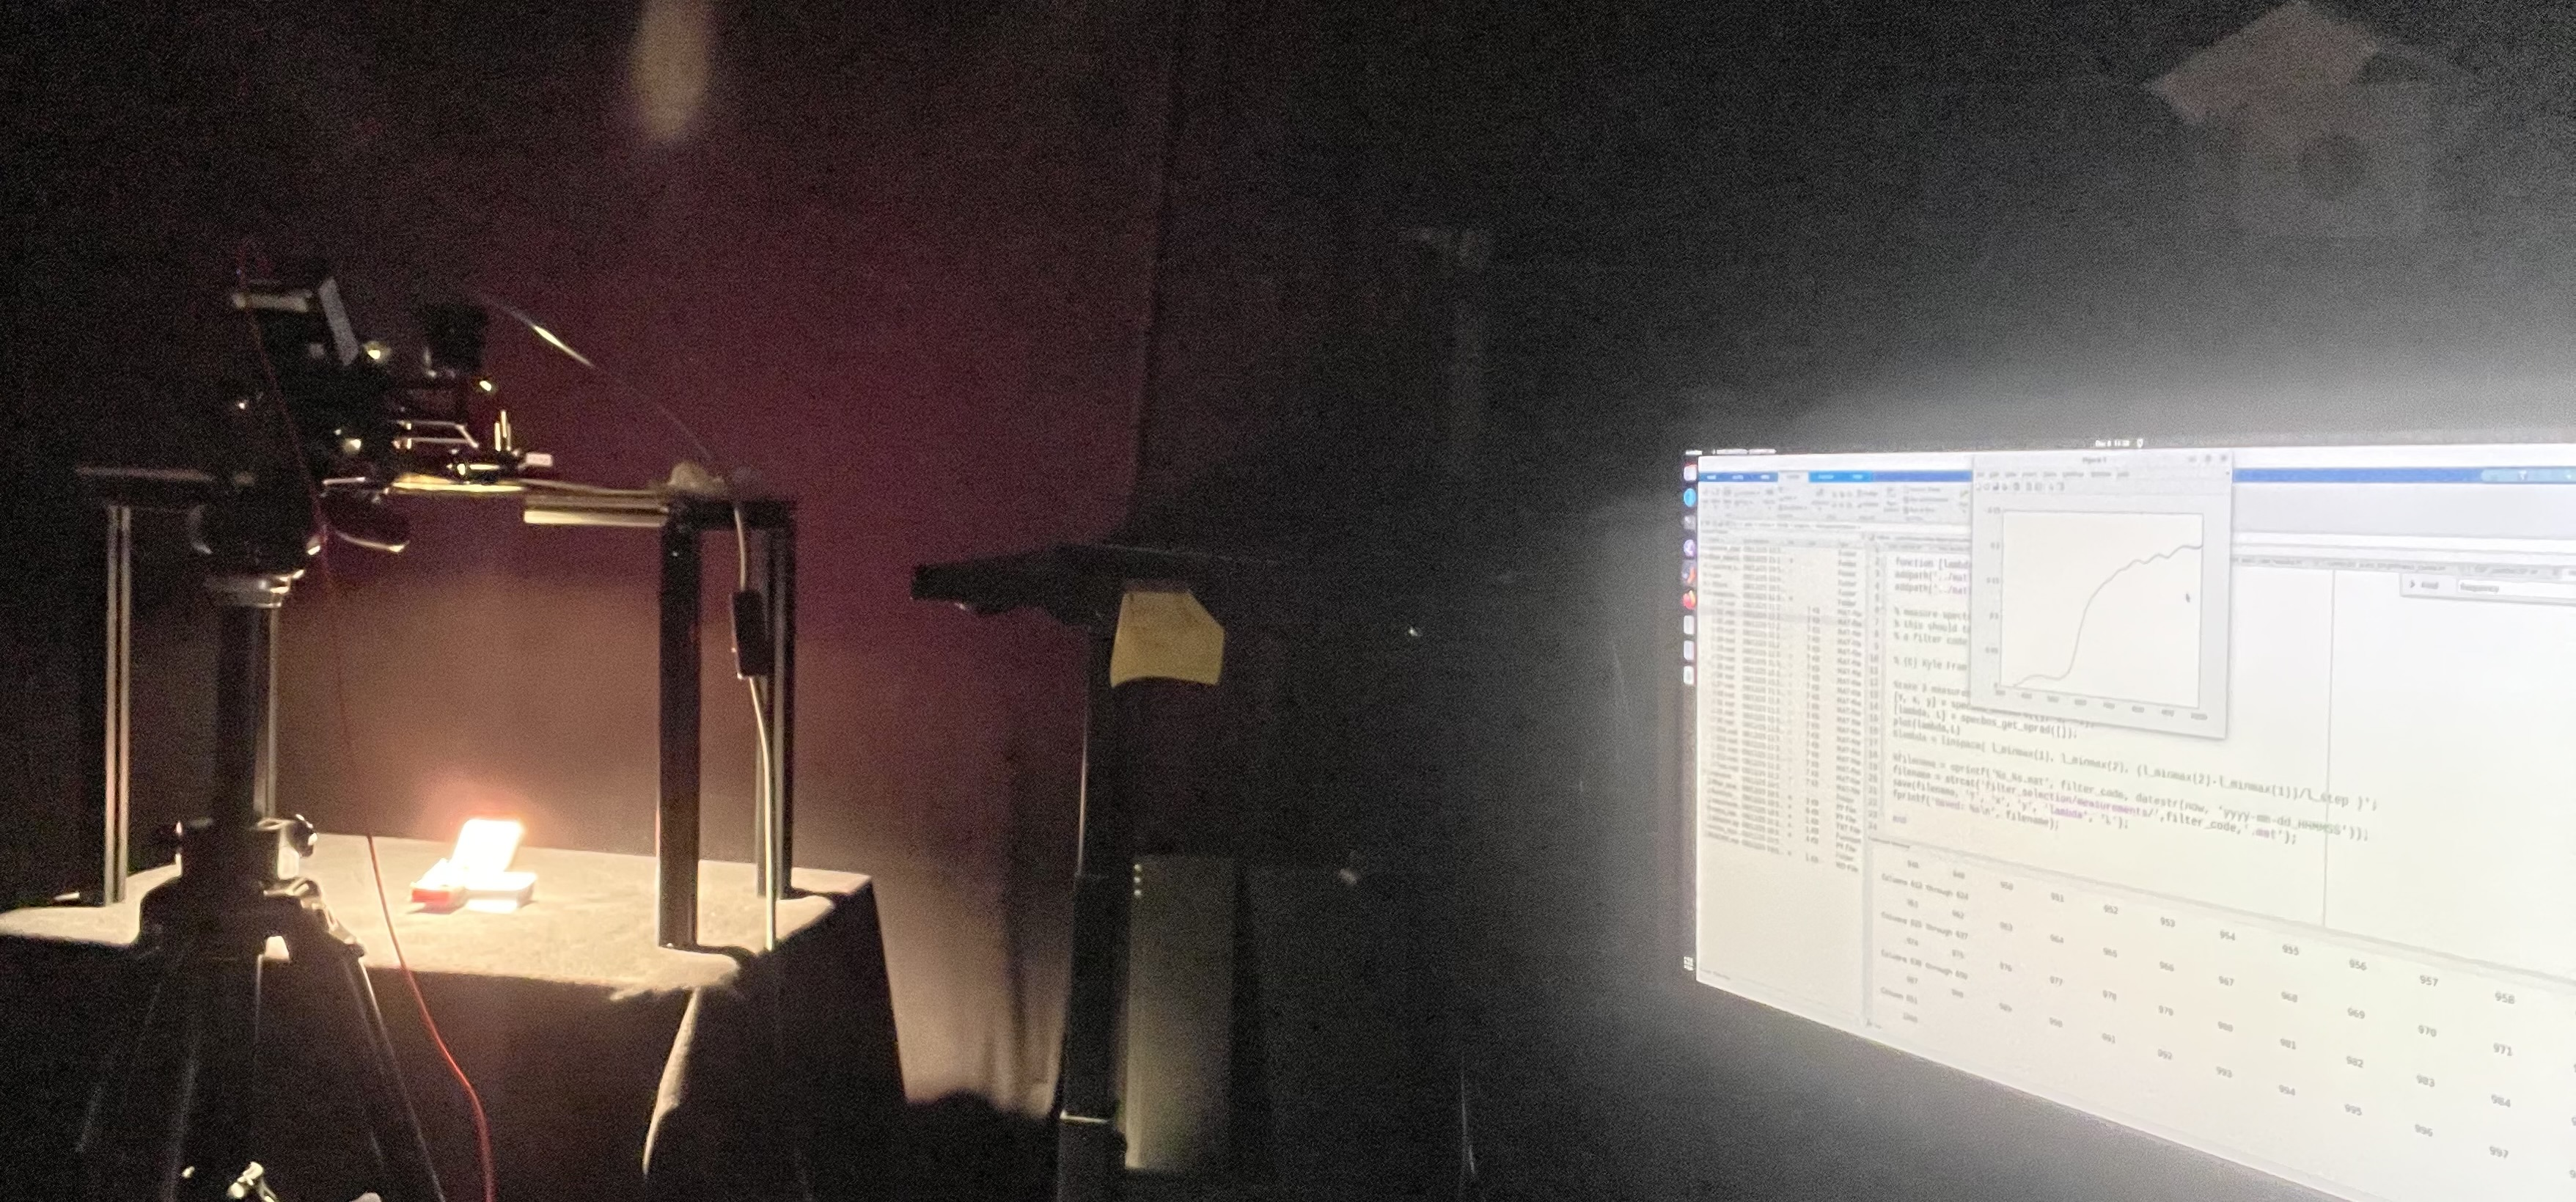
\includegraphics[width=\linewidth]{media/Measure3.jpeg}
    \caption{Computer readout of spectrophotometer measurement in dark room}
\end{figure}

For our target functions, we utilize the UCL Color \& Vision Research Laboratory repository of cone and rod sensitivity functions \cite{CVRL}, including CIE XYZ 1931 and CIE 2006 LMS functions (transformed to XYZ for consistency).

We also benchmark our performance by computing $\Delta E_{2000}$ using the RGB coordinates of the Macbeth ColorChecker as per Pascale \cite{Pascale2006RGBCO}. 
For a demonstration of color reconstruction across scenes, we utilize the CAVE dataset from Yasuma et al. \cite{yasuma2010generalized}

\begin{figure}[H]
    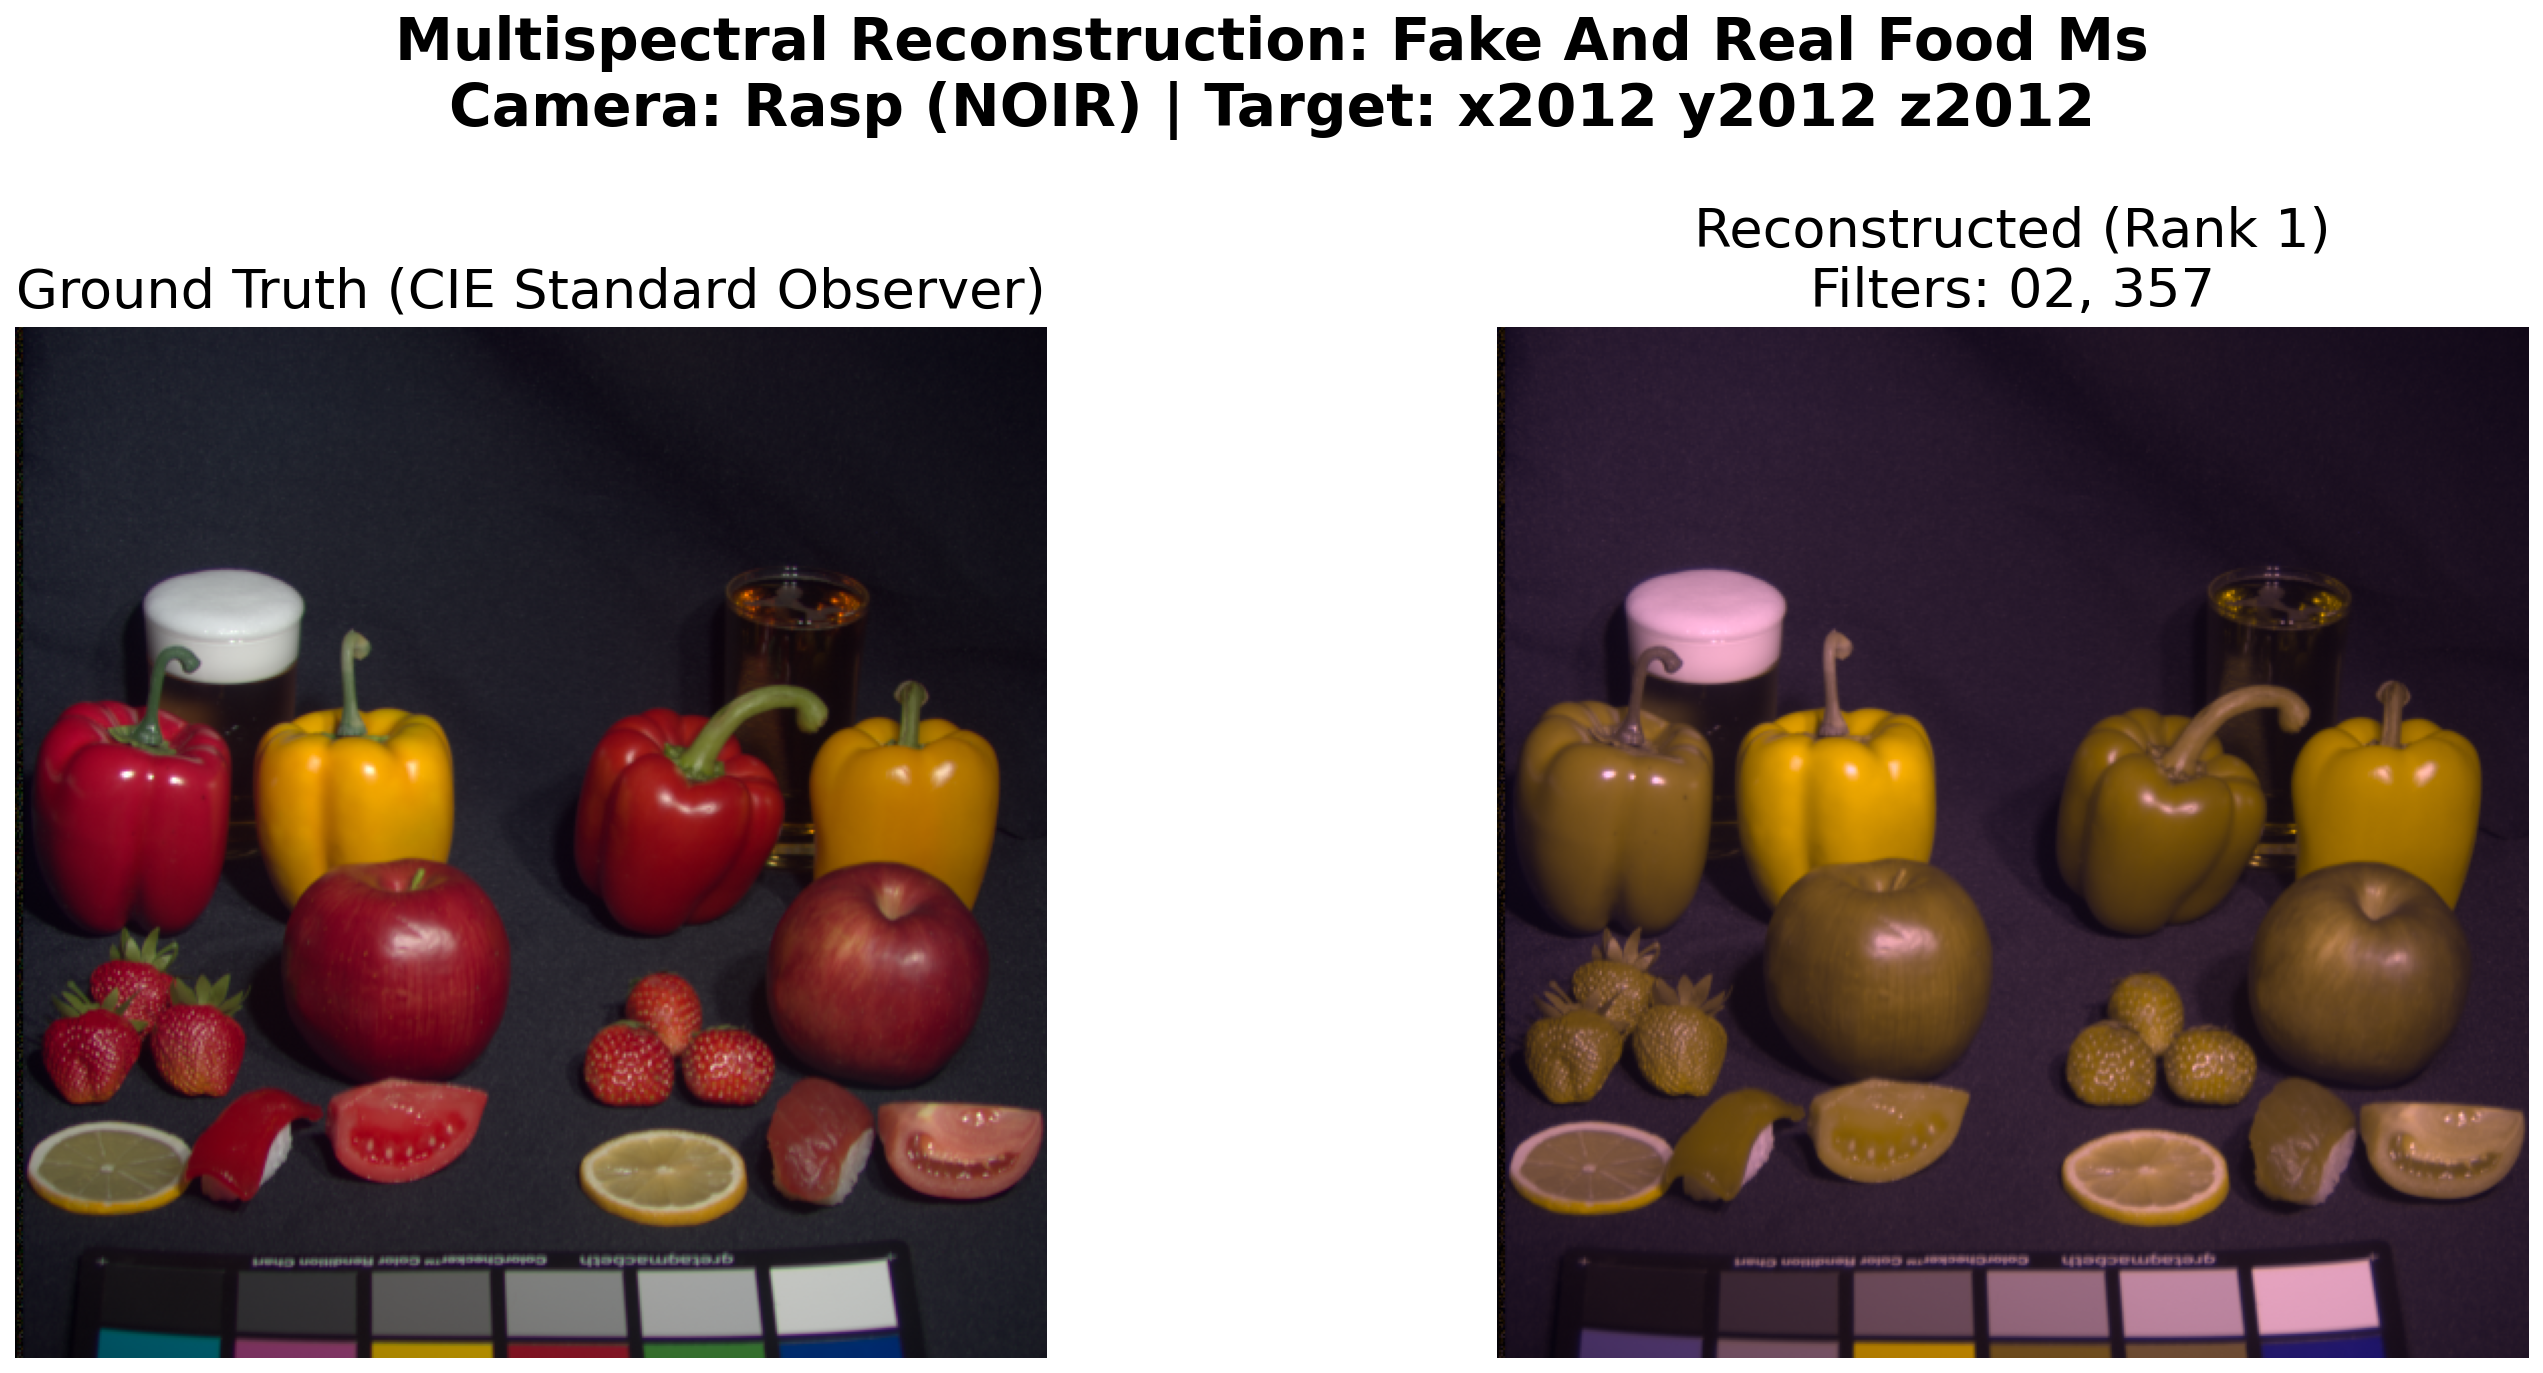
\includegraphics[width=\linewidth]{media/Cave_DataCollection.png}
    \caption{Example of a simulated reconstruction from the CAVE dataset for $k=2$ filters}
\end{figure}

Next, we replicate the above simulated spectral reconstruction in the lab, capturing a scene including one Preferred Memory Color Chart \cite{ThouslitePMCC} under the same Lilliput illuminant \cite{UtopiaCamLiliput}.


\begin{figure}[H]
    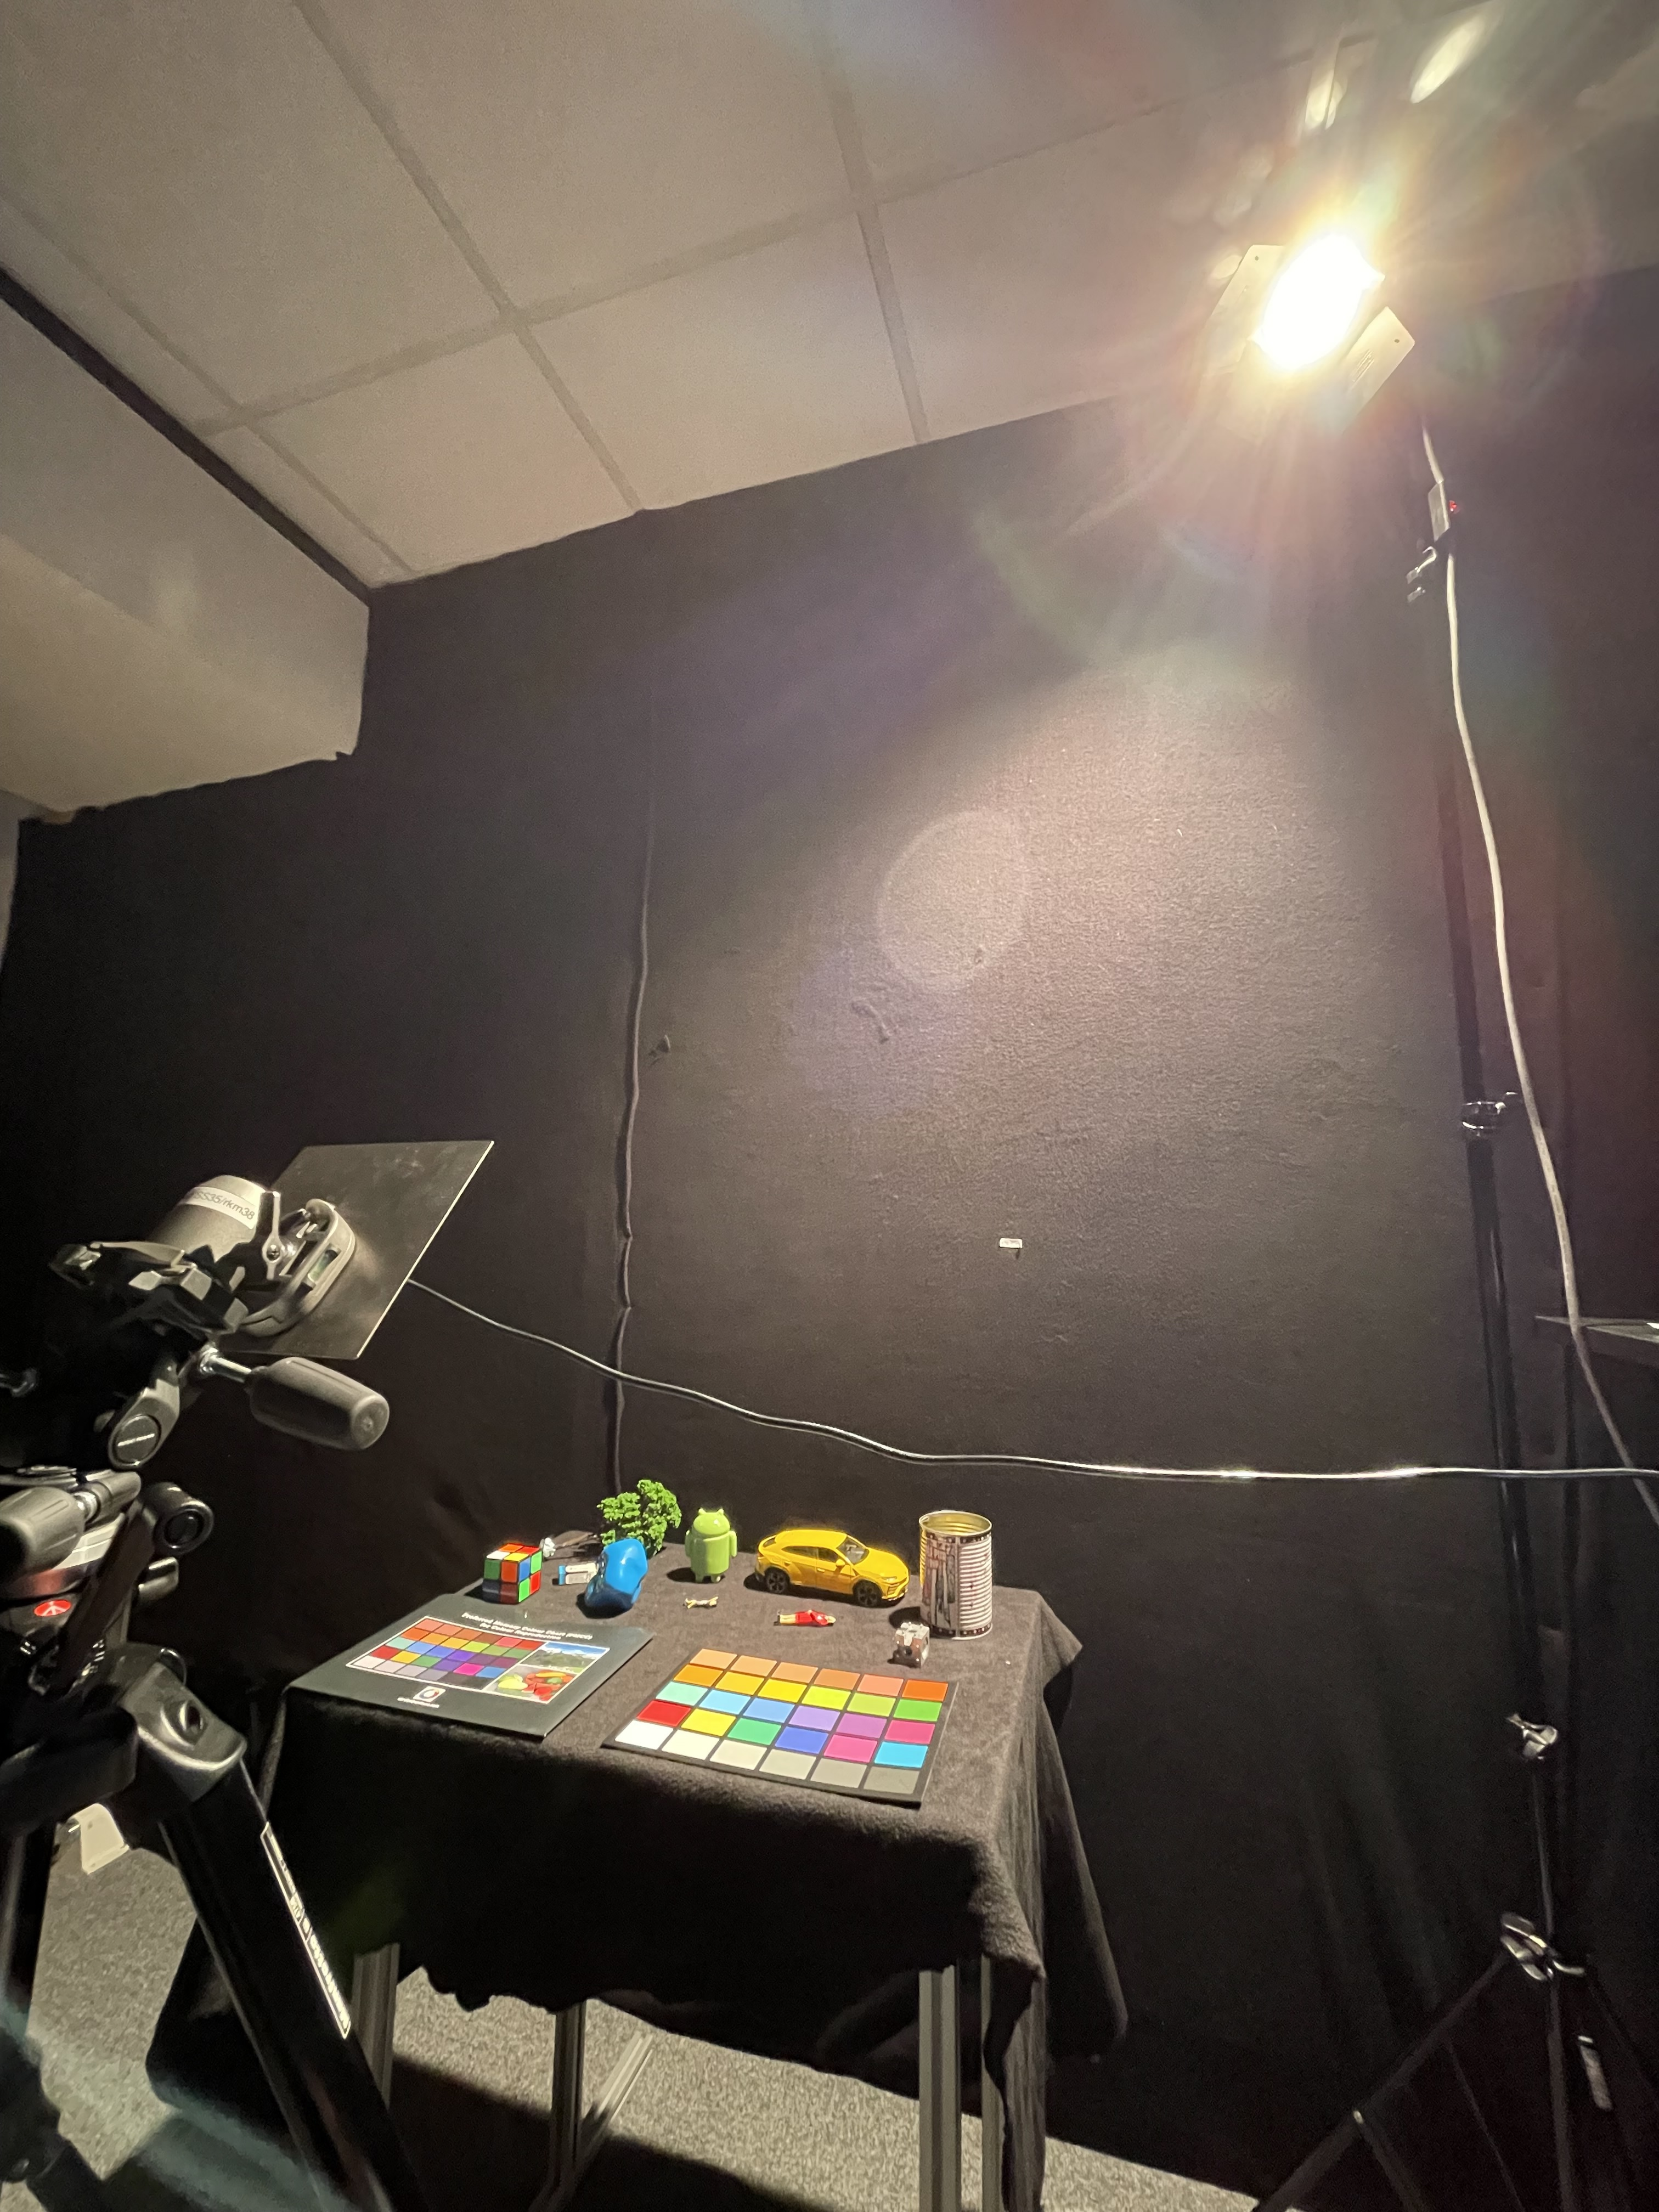
\includegraphics[width=\linewidth]{media/spectralLab.jpeg}
    \caption{Lab setup for multispectral imaging with illuminant}
\end{figure}

To this end, each filter was placed in front of the camera, mounted onto a tripod and aimed at a scene including objects of different reflectances and colors. 
Additionally, the PMCC was placed at the front of the scene for easy quantitative color analysis. 
The camera was kept in place such that we could pick one pixel per capture for which to measure each color patch under each respective filter. 

\begin{figure}[H]
    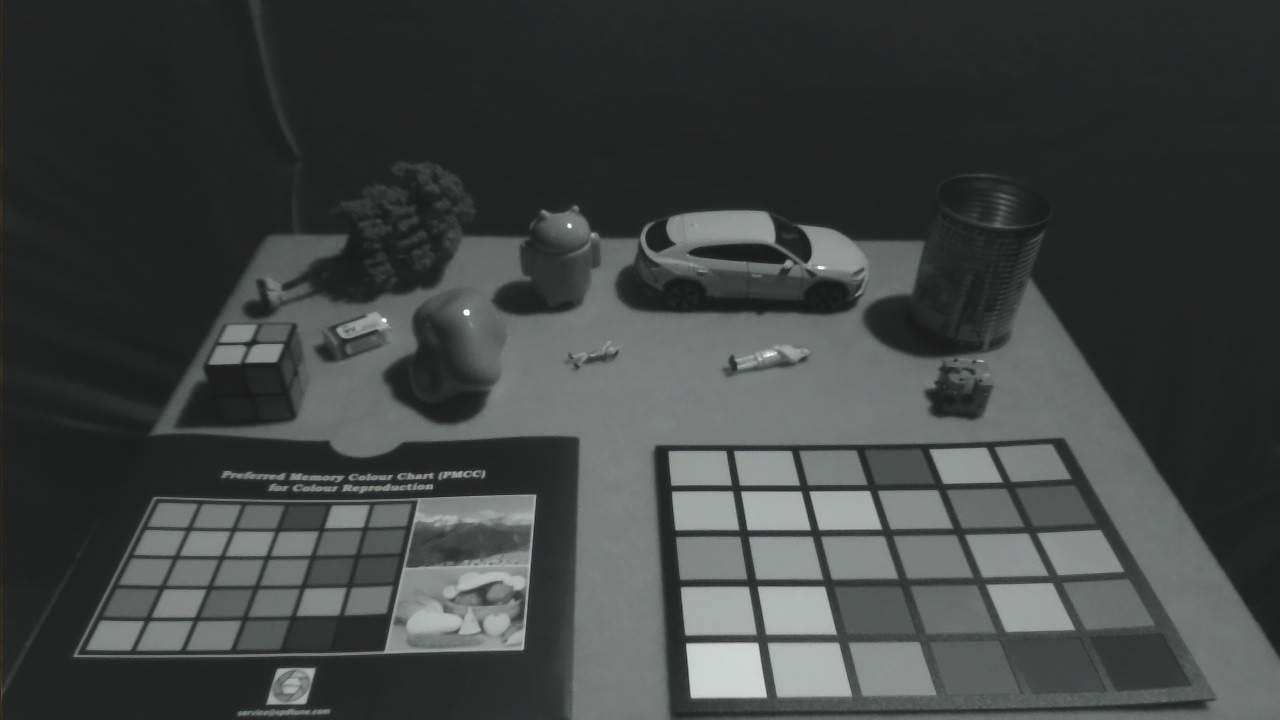
\includegraphics[width=\linewidth]{media/398.jpg}
    \caption{Capture of filter \#398 from monochrome camera, including PMCC in the foreground}
\end{figure}

Other items were placed in frame as well for qualitative reivew, a subset are shown in detail. 

\begin{figure}[H]
    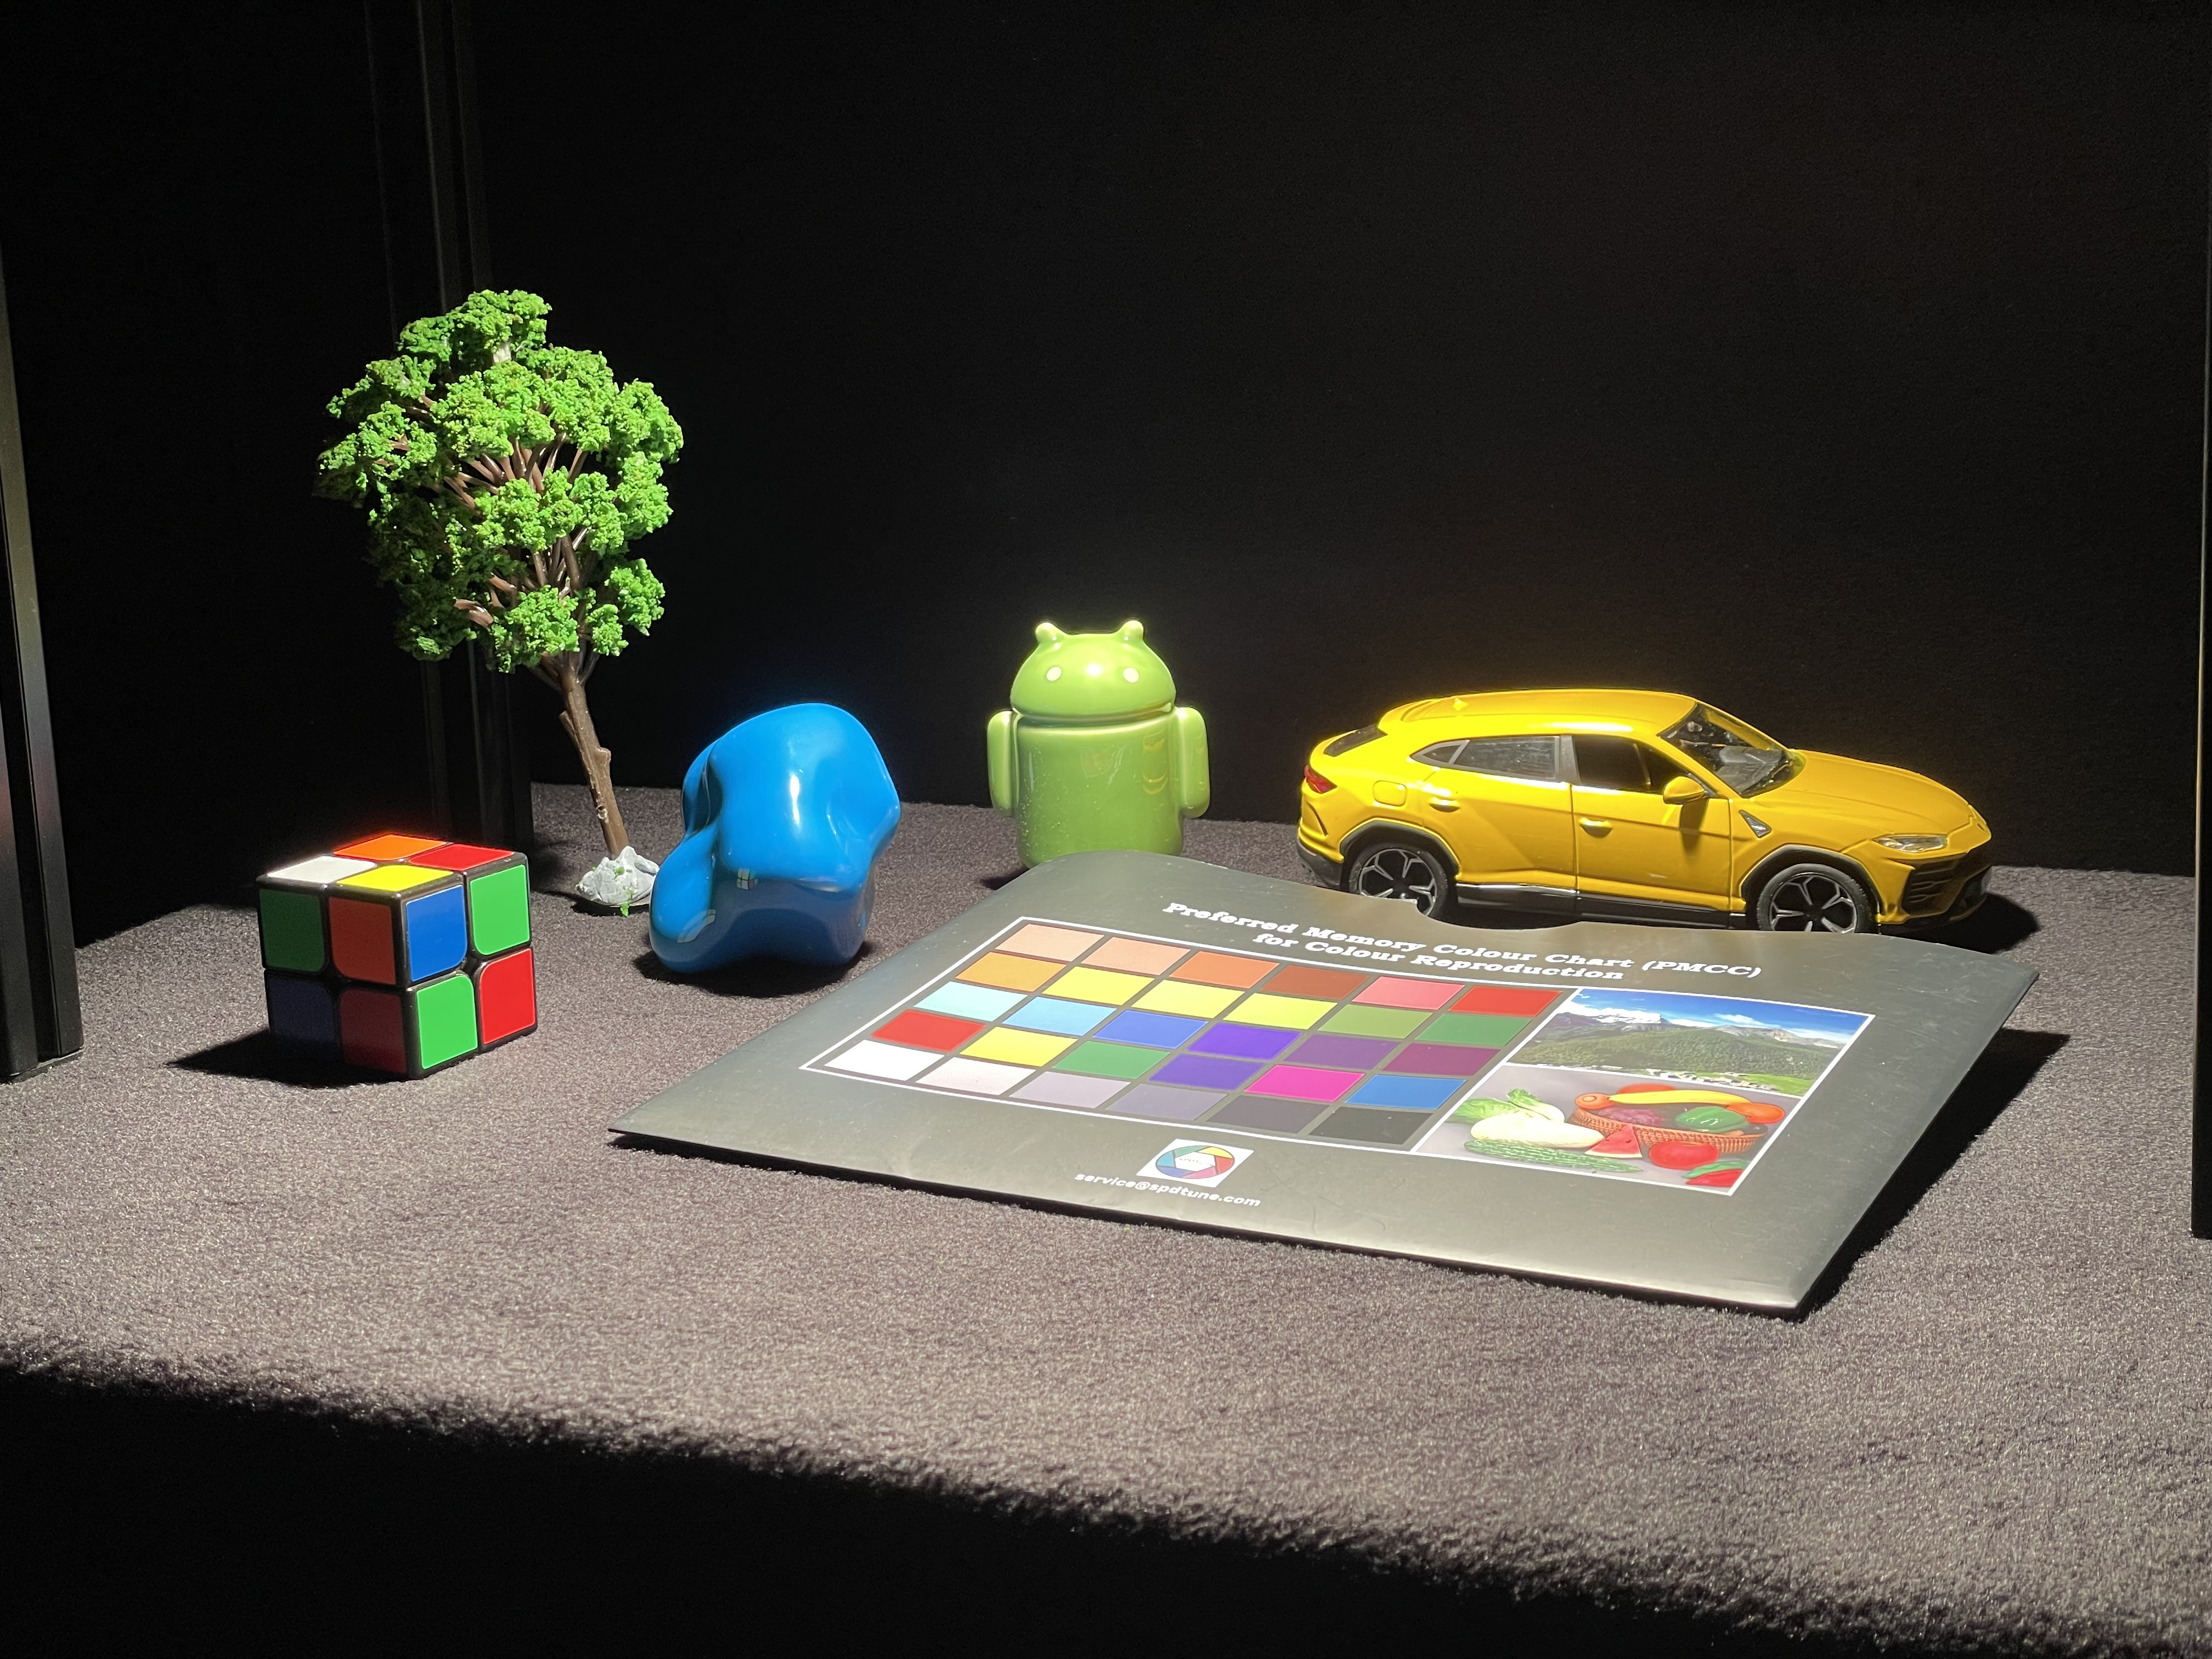
\includegraphics[width=\linewidth]{media/items.jpeg}
    \caption{Subset of items staged for color capture}
\end{figure}

Ground truth measurements were taken with the same spectrophotometer as above, under consistent angular setup and the same lighting. 
Each panel of the SPD was captured in order to compute absolute colorimetric difference between spectral reconstruction and ground truth. 

\begin{figure}[H]
    \includegraphics[width=\linewidth]{media/Spectrophotometer2.jpeg}
    \caption{Items staged for color capture, including a PMC}
\end{figure}

A render of the readings taken with the spectrophotometer is shown, providing a human-eye check that our readings were taken correctly. 
The white patch provided a white point and other patches were rendered after normalizing to this white, taking the illuminant as D65.
\begin{figure}[H]
    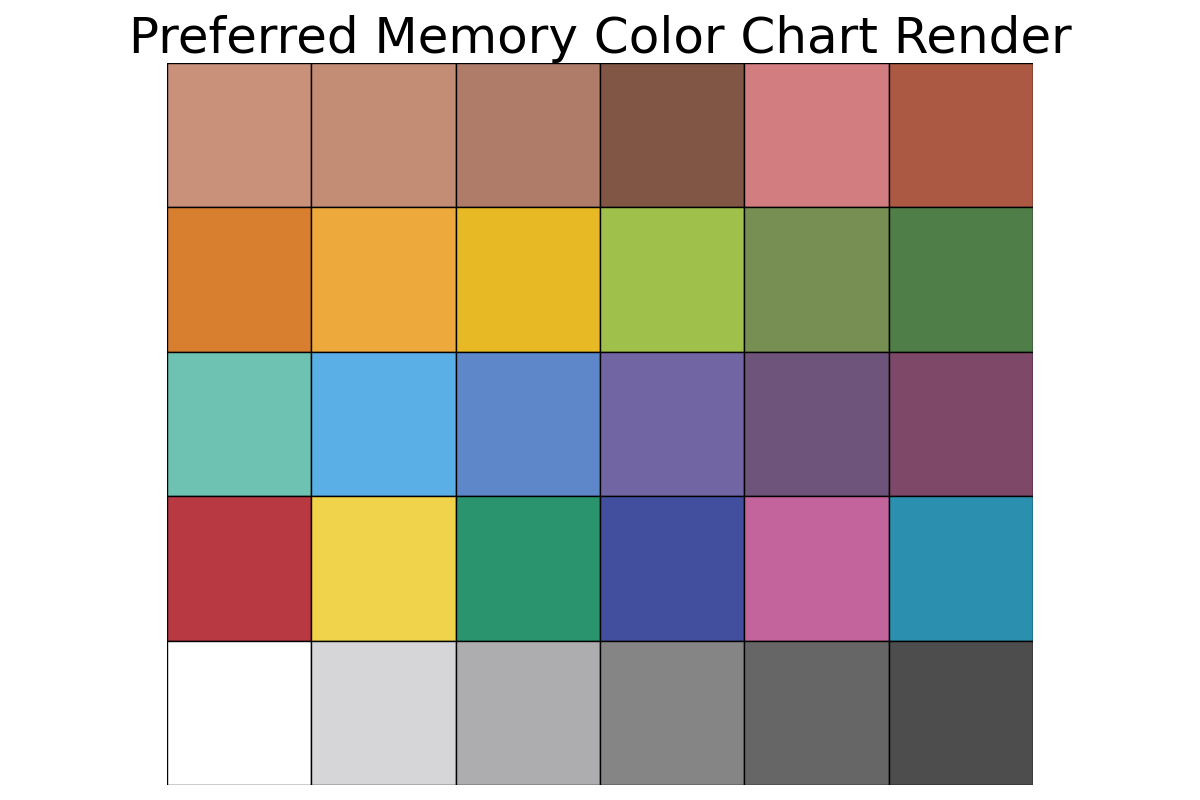
\includegraphics[width=\linewidth]{media/colorcheck_render.png}
    \caption{Render of Spectrophotometer Readings}
\end{figure}

We plot the color patches on the standard XYZ gamut for illustration.

\begin{figure}[H]
    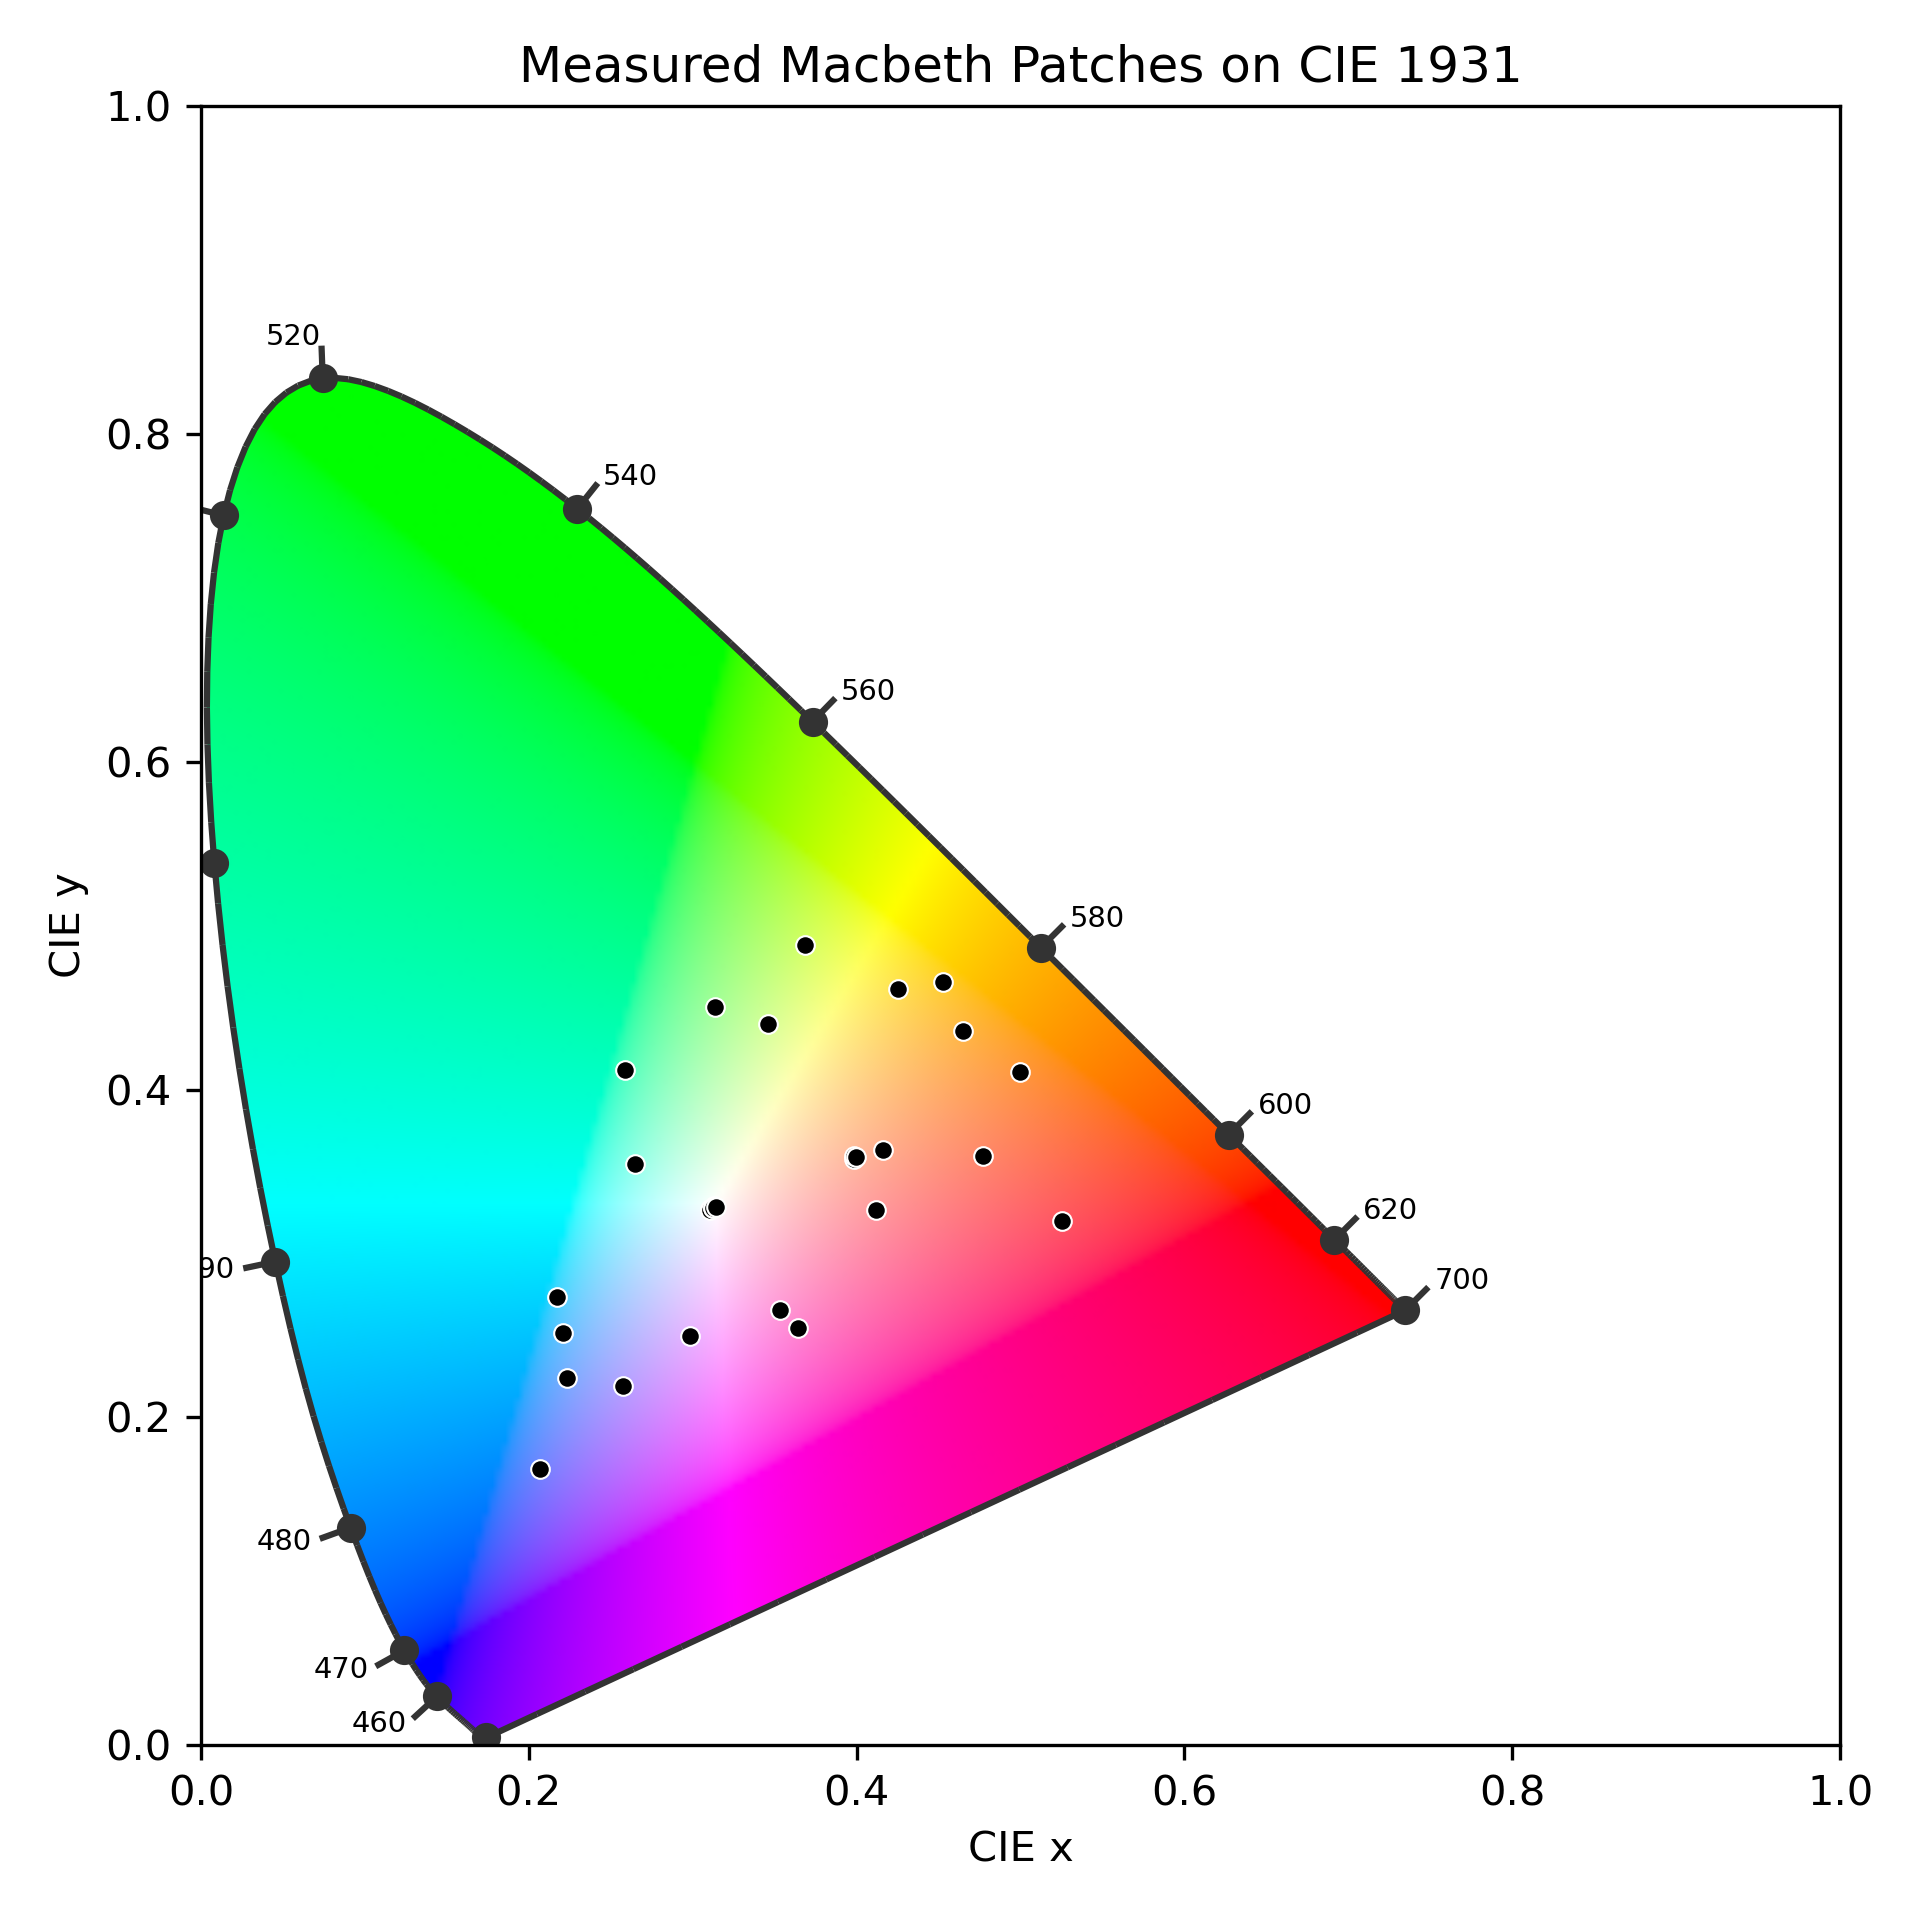
\includegraphics[width=\linewidth]{media/colorcheck_chromacity.png}
    \caption{Distribution of patch locations on the CIE 1931 Color Gamut}
\end{figure}


\subsection{Problem Formulation}

For approximations of XYZ, we follow the work of Hardeberg \cite{Filterselection} in adopting MSE between target and simulation over the visible spectrum as the loss function and minimizing loss via search for an optimal $\boldsymbol{M}$.
%Abstractly, we denote the loss function $L(\boldsymbol{x}(\lambda),\boldsymbol{y}(\lambda))$ for arbitrary target $\boldsymbol{x}(\lambda)$ to be approximated by the estimation (i.e. combination of filter wheel sensitivities) as $\boldsymbol{y}(\lambda)$ (to be solved for) defined over the domain $\lambda \in \omega$. 

\begin{equation}
    L({X_c}(\lambda),{\rho}_{c,k}(\lambda)) = \int_{\omega}\|{X_c}(\lambda)-{\rho}_{c,k}(\lambda)\| d\lambda
    \label{eq:5}
\end{equation}

%% Kyle, why not put x rather than t
%%% - KYLE: this statement is redundant and adds confusion, likely easier to omit.
%%%We take $t \in \{X,Y,Z\}$ as our target color matching functions and 
%% Kyle added y(\lambda)=
%%%$y(\lambda)=\rho'_c(\lambda)$ with $c\in \{R,G,B\}$ as our simulated functions. 
We consider loss from all color channels equally. Given that we are limited by 1 nanometer steps in measurement, we discretize over $\omega$, taking $\omega_d = \{400,401...750\}$. We sum MSE over $\omega_d$ to compute our total error, and then sum over each response function:

\begin{equation}
    L_d({X_c}(\lambda),\rho_{c,k}(\lambda)) = \sum_{\lambda \in \omega_d}\|{X_c}(\lambda)-{\rho}_{c,k}(\lambda)\|
    \label{eq:6}
\end{equation}

We minimize loss by selection of $k$ representing our $N$ `active' filters (which incorporate the intrinsic sensitivity of a grey-scale sensor) each having transmission functions ${f}_k(\lambda)$ (thus comprising a $k$ length vector of functions), and $\boldsymbol{M}$, a $3\times k$ color correction matrix. 
We also define $\underline{X}(\lambda)$ as the $X,Y,$ and $Z$ functions, and $\underline{\rho}$ as the corresponding simulated response functions, with $\underline{f}(\lambda)$ as the stacked $f_k(\lambda)$ functions. 

\begin{equation}
    \argmin_{\mathbf{M}} \sum_{\{X,Y,Z\}} L_d(\underline{X}(\lambda),\underline{\rho}(\lambda))
    \label{eq:7}
\end{equation}


%In this case, the optimal weights can be found using the pseudo-inverse \cite{greville1960some, BEUTLER1965451, macausland2014moore}.
We define $\boldsymbol{F}$ as the $k\times 351$ matrix $\underline{f}(\lambda)E(\lambda)S(\lambda)$ at each $\lambda \in \omega_d$. 
And the discrete set of $3 \times 351$ XYZ functions as $\mathbf{X}$. 
If we find a good minimization according to our loss function, then

\begin{equation}
    \boldsymbol{X} = \boldsymbol{M}\boldsymbol{F}
\end{equation}  

Using a least-squares loss we can solve for $\boldsymbol{M}$, in closed form, using the Moore-Penrose pseudo-inverse \cite{greville1960some, BEUTLER1965451}, denoted $A^+$ for a matrix $A$. 
The unique $351 \times k$ Moore-Penrose pseudo-inverse solution $\boldsymbol{F}^+$ has the desirable property that while we may not exactly satisfy the Luther condition, it provides the closest possible approximation for a given filter set $k$ \cite{macausland2014moore}:
\begin{equation}
    \boldsymbol{M} \approx \boldsymbol{X}\boldsymbol{F}^+
\end{equation} 

As a point of detail we must alter this optimization if any of our filters have 0 transmission in a part of the assumed wavelength interval. 
The NOIR filter only has nonzero transmittance in [400,650] nanometers. 
So, when this filter is used we can only optimize within this wavelength interval.
%Note that for algorithmic stability of the pseudoinverse, we must truncate to $\lambda \in \{400,401...650\}$ when using the $NOIR$ filter. 

Further, we consider applications using loss functions $L$ and their respective $L_d$ which may not be the MSE loss. 
We consider SMAPE and log-loss functions amongst others, for which analytical solutions do not necessarily exist. 
For these, we use a gradient descent algorithm with initial guess informed by the Moore-Penrose pseudoinverse.

As an extension of the above, we model the noise of our camera using a modified MSE loss plus an error term. 
Following Hanji \cite{hanji2020noise}, we model camera photon registration as a poisson process. 
Borrowing the terminology, we take the radiance at each pixel $p$ as $\phi(p)$, having pixelwise radiance defined as $R(p)~Pois(\phi(p)t)$.
Then, with gain $g$ and exposure time $t$, he expected scene radiance and variance, or noise, are determined by
\begin{equation}
    E(R(p)) = \phi(p)tg 
\end{equation} 
\begin{equation}
    V(R(p)) = E(R(p))g 
\end{equation} 
Thus, our photonic camera noise, V(R(p)) is a linear function of exposure time. 
We provide a study in reconstruction quality as a function of 'shutter speed,' which refers to the duration of capture per filter. 
This is again implemented by defining $L = MSE + V(R(p))$, which can be achieved with a few steps of gradient descent from the MSE pseudoinverse solution. 

\subsection{Filter Selection}

While the number of filters $M$ may be large, we ideally would posit a filter wheel with fewer filters.
Some works, such as Finlayson and Zhu \cite{finlayson2020designing} aim to construct optimized filters for camera and illumination spectifics. 
However, off-the-shelf gel filters provide a cost effective tool, if a good selection can be made. 
We take $k$, the number of filters chosen from the $M$ sized universe, as well as $L$, the loss function as per the above.

The problem of filter selection and $\boldsymbol{M}$ computation are closely related. 
For non-brute force methods of filter selection, we effectively 'guess' the combination that might produce the best MSE after choosing $M$.
This lends itself to either exclusion or inclusion algorithms, the former we refer to as LASSO, the latter as PCA, 


\subsubsection{Brute Force Search}
In the naive solution, we find the optimal filter combination for every subset of $k$ filters (where $k$ is small) drawn from the $M$ filter set by selecting the combination with the lowest loss, considering all combinations of filters (there are nearly 10,000,000 of these for $k=5$). 
In Figure 2 we plot the errors across all sets of 5 filters (multiplied by the camera sensitivity) from the worst to best performing quintuple. 
We compute the Moore-Penrose pseudo-inverse for each set of filters. 
Our implementation is parallelized over 8 NVIDIA L4 GPUs, with a combined pool of up to 192GB VRAM, enabling us to compute brute force searches of $k=5$ in approximately 7 minutes. 
%% Kyle N=5?

\begin{center}
    \label{fig:errors}
    \centering
    \includegraphics[width=\linewidth]{media/all_errors.png}
    \captionof{figure}{MSE Error distribution across all filter combinations for k=5}
\end{center}

As the search space experiences combinatoric explosion with $N$, we cannot feasibly consider all combinations for large $N$.
To alleviate this issue, we introduce a 'prune' factor which removes filters based on a cosine similarity metric. 
Given that our brute force method aims to provide a ground truth in which to compare performance of other filter selection algorithms, we allow the pruning of filters in the same way for other algorithms. 

\subsubsection{PCA Analysis}

To find the optimal filter combination
%for each $N$ 
without brute force search, we can use PCA analysis to find approximate solutions. 


This method initially creates one $3\times M$ matrix $\boldsymbol{M}$ and iteratively selects until reaching $k$ filters and thus our final $3 \times k$ matrix of weights. 
Specifically, the selection is performed by projecting $\boldsymbol{F}$ onto the space spanned by the target $\boldsymbol{X}$ matrix, finding the filter with the highest norm as per the Matching Pursuit method outlined in Mallat and Zhang \cite{mallat1993matching}.
We iteratively apply this methodology $k$ times, each time on a subset of the resultant orthonormal basis formed by subtracting the selected filter's projection.

This method is comparatively fast, able to compute the $k=5$ case in 19 seconds on a single L4 GPU. 
This method also scales well, with $k=8$ runtime at only 20 seconds. 

We show the relative timings for Brute Force and PCA algorithms below. 
\begin{center}
    \centering
    \includegraphics[width=1.05\linewidth]{media/timing_comparison.png}
    \captionof{figure}{Timing Comparison between PCA and Brute Force Selection Methods}
\end{center}

However, we note the improved MSE result for the brute force selection methodology.
\begin{center}
    \centering
    \includegraphics[width=1\linewidth]{media/mse_comparison_exact_paths.png}
    \captionof{figure}{MSE Comparison between PCA and Brute Force Selection Methods, $k_2=0$}
\end{center}

\subsubsection{PCA Analysis with Macbeth Target}

In the original PCA Matching Pursuit as outlined above, we have an underdefined problem for $k>3$, as our 3 dimensional target space may be nearly spanned by the projection of the first 3 filters. 
One way to mitigate this issue is to project our space onto that as defined by the Macbeth Color Checker patches. 
Using this methodology, we define a higher-dimensional space and thus a lower incemental value per added filter, with a better result at high $k$. 
However, we will observe that this technique only accurately reproduces human eye color matching functions such as the CIE XYZ family of functions, and fails to generalize to other applications. 
That being understood, this method is able to achieve better metrics at high $k$. 
For practical purposes, the difference is immaterial due to the cost of increasing $k$ above 10 or so, in terms of size of components and the capture time increase inherent to adding additional filters. 
\begin{center}
    \centering
    
\includegraphics[width=1\linewidth]{media/placeholder.jpg}
    \captionof{figure}{Placeholder for comparison of MSE/DeltaE at high $k$}
\end{center}

\subsubsection{LASSO Selection}
This method performs 'dropout' from a matrix $\boldsymbol{M}$ defined as the entire universe of filters. 
It then iteratively tunes the values of said matrix, dropping out columns with a low norm such that the filter is not meaningfully used in reconstruction.
The loop runs until only $k$ filters remain.

\begin{center}
    \centering
    
\includegraphics[width=1\linewidth]{media/placeholder.jpg}
    \captionof{figure}{Placeholder for LASSO}
\end{center}

\subsubsection{Brute Force Search Augmented PCA} 

$\;$\newline While brute force methods guarantee minimum possible error by investigating the entire search space, large $k$ implementations render this technique impractical. 
Additionally, our PCA method outlined above cannot always identify the optimal filter set, and has a nonnegligible MSE shortfall vs. exhaustive search for all $k>1$.

To address this problem, we use a blended method which finds a PCA solution for $k_1$ filters, and then considers all further possible combinations from a further $k_2$ filters, for a total $k=k_1+k_2$. 
This provides a middle ground to the performance-accuracy tradeoff.
There is negligible MSE difference between brute force and PCA methods at $k_2>1$ for all $k_1$.
Further, for $k_2<4$, the added time from the exhaustive search step is between 5-20 seconds on the 8 aforementioned L4 GPUs.
%We note here that the MSE shortfall observed above has mostly disappeared, with PCA having a significant performance improvement over Brute Force.
%A full performance overview is included in the Appendix (\ref{tab:timing_comparison}).
\begin{center}
    \centering
    \includegraphics[width=\linewidth]{media/mse_comparison_exact_paths_n2_2.png}
    \captionof{figure}{MSE Comparison between PCA and Brute Force Selection Methods, $k_2=2$}
\end{center}

One challenging problem introduced by the extra choice of $k_2$ is an explosion of state space. 
Whereas in the original problem, we have a reliably monotonically decreasing relationship between MSE and $k$ in the brute force case (if the 'best' filter would decrease MSE, a weight of 0 would be applied), the introduction of the brute force rounds requires us to intellegently choose $k_2$. 
Then, under practical considerations in a filter wheel of limited $k$, the choice of $k_1$ vs. $k_2$ becomes a difficult to define and hard to optimize tradeoff.
In fact, certain artifacts emerge in the comparison between brute force and heuristic algorithmms with $k_2>1$, such as improved MSE performance for the PCA algorithm at $k=2$ as shown above. 

Presumably a brute force algorithm would necessarily find the global minimum MSE, however, with $k_2>0$ and the brute force solution 'branching' (in essence, considering $k_2$ filters from the $k_1$ brute force filters) may miss the optimal filter combination. 
Therefore, any brute force solution with $k_2>0$ should be considered with caution. 
There is value in augmenting a brute force solution, as runtime is greatly reduced, but we find that the effect of mixing search algorithms at an intermediate value provides an efficient yet accurate middle ground for practical values of $k$.

